
\documentclass[journal,12pt,twocolumn]{article}
\usepackage{graphicx}
\graphicspath{{./figs/}}{}
\usepackage{amsmath,amssymb,amsfonts,amsthm}
\newcommand{\myvec}[1]{\ensuremath{\begin{pmatrix}#1\end{pmatrix}}}
\usepackage{listings}
\usepackage{watermark}
\usepackage{titlesec}
\let\vec\mathbf

\titlespacing{\subsection}{0pt}{\parskip}{-3pt}
\titlespacing{\subsubsection}{0pt}{\parskip}{-\parskip}
\titlespacing{\paragraph}{0pt}{\parskip}{\parskip}
\newcommand{\figuremacro}[5]{
    
}
\lstset{
frame=single, 
breaklines=true,
columns=fullflexible
}
\thiswatermark{\centering \put(1,-75){
\includegraphics[scale=0.5]{iith.png}} }

\sloppy
\title{\mytitle}
\title{
Matrix Assignment - Conic
}
\author{mohammad imran}
\begin{document}
\maketitle
\tableofcontents
\bigskip


\section{\textbf{Problem}}
Tangent to the curve y=$x^2+6$ at a point (1,7) touches the the circle $x^2+y^2+16x+12y+c=0$ at a point Q then the coordinates of Q are ?. \\


\section{\textbf{Solution}}
The equation of a curve  is given as,  
\\
        $y=x^2+6$ \\
        
 the above equation can be expressed in the form  \\    
${\vec{x^{\top}V x} + 2\vec{u^{\top}x}} + f=0$
\\

where,
\\

$\vec{V}=\myvec{1&0\\ 0&0}$ and $\vec{u}=\myvec{0\\\frac{-1}{2}}$and f=6
\\

for the given conic
\\

the point where the tangent touches the conic is $Q(1,7)$\\
\\
given a point of contact Q,  then Equation of tangent is given by,
\\

$\vec{(VQ +u)^{\top}}\vec{x} + \vec{u^{\top}Q} + f = 0$
\\
\\


$\vec{(VQ)}^{\top}\vec{x} = -f$
\\
\\
which can be written as 
\\

$\vec{n}^{\top}\vec{x} = C$
\\
\begin{equation}
\myvec{2 & -1}\vec{X}=-5
\end{equation}
\\

$n=\vec{VQ} = \myvec{2\\-1}$ and $C=f=-5$
\\

from equation of line we can write directional vector\\
\\$\vec{m}=\myvec{1\\2}$
\\

given circle equation\\
\\
$x^2+y^2+16x+12y+c=0$\\
\\
the above equation can be expressed as
\\
${\vec{x^{\top}V x} + 2\vec{u^{\top}x}} + f=0$
\\
where
\\

$ \vec{u}=\myvec{8\\6} $
\\ 
the point of intersection of the line with the conic section is given as
\\
\begin{equation}
\vec{x}=\vec{q}+\mu\vec{m}
\end{equation}\\
where, 
$\mu=\frac{1}{\vec{m}^{T}\vec{v}\vec{m}}(-\vec{m}^{T}(\vec{v}\vec{q}+\vec{u}))$\\
\\
by substituting all the values we get\\
\\
$\mu$=-7
\\ \\
as we have point of contact q and directional vector m and $\mu$
\\ \\
by substituting all the values  in eq 2 we get point of intersection on the line\\
\\
$\vec{X}=\myvec{-6 \\ -7}$
\\

\section{\textbf{Figure}}
\begin{figure}[h]
    \centering
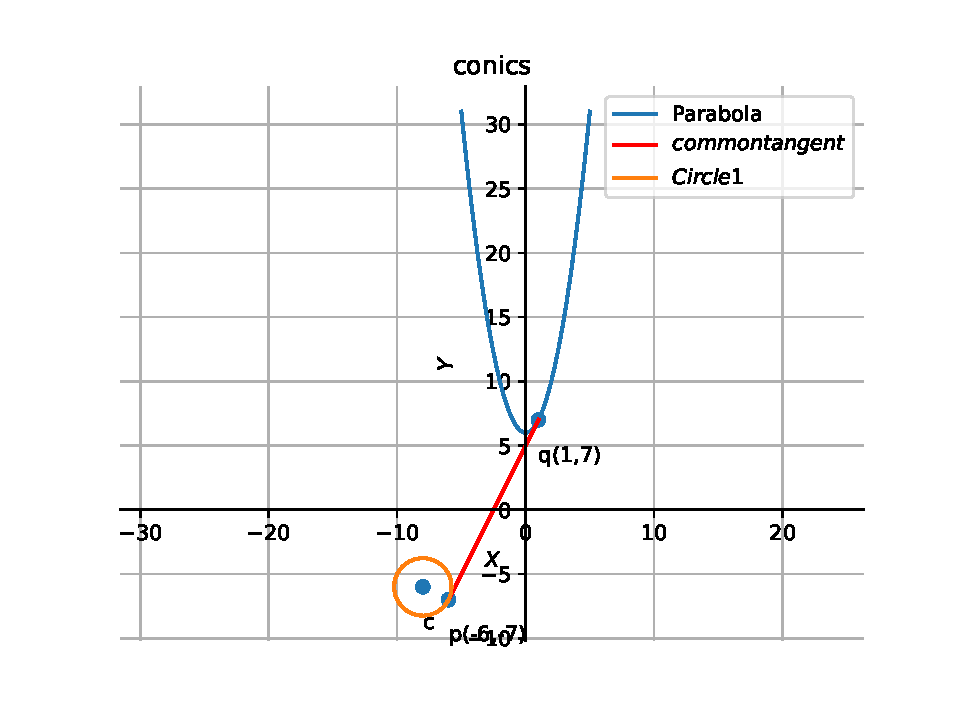
\includegraphics[width=\columnwidth]{figconic1.pdf}
    \label{fig:my_label}
\end{figure}


\section{\textbf{Code Link}}

\begin{lstlisting}

 https://github.com/imran111888/fwc2/tree/main/matrix/conic/codes

\end{lstlisting}
Execute the code by using the command\\
\textbf{python3 conic.py}



\end{document}
